%!TEX root = main.tex

\begin{figure}[!tb]
	\centering
	{
	\newcommand\myheight{0.145}
	\subfloat[] {
		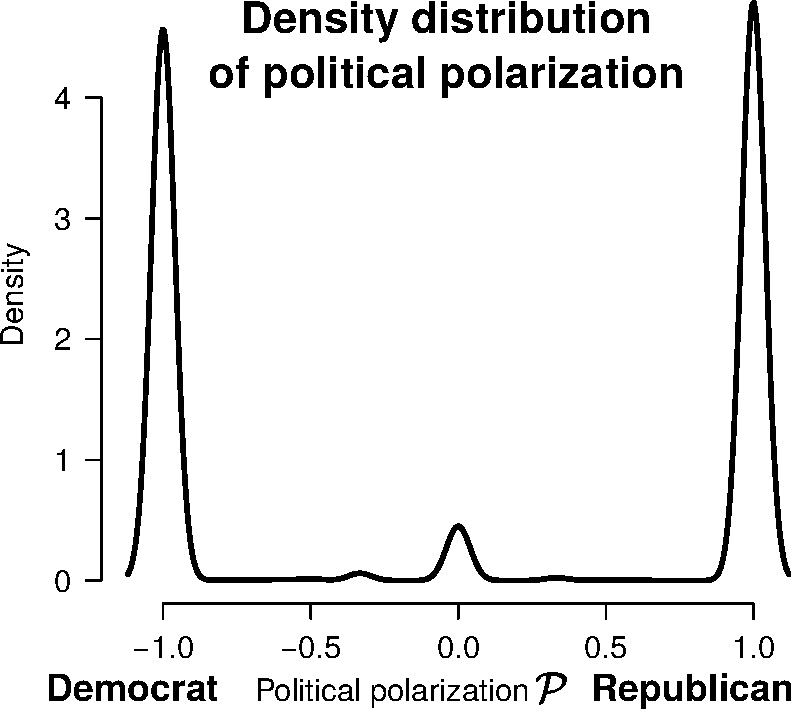
\includegraphics[height=\myheight\textheight]{a-density-distribution-political-bias}
		\label{subfig:distribution-political-bias}
	}
	\subfloat[] {
		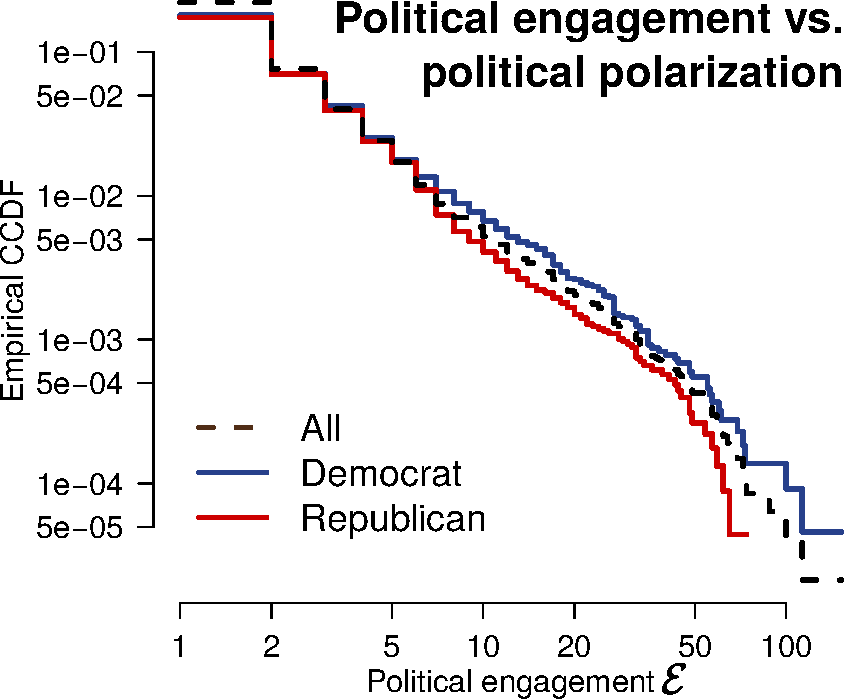
\includegraphics[height=\myheight\textheight]{b-CCDF-bias_engagement-vs-political-bias}
		\label{subfig:engagement-vs-political}
	}}
	\\
	{
	\newcommand\myheight{0.16}
	\subfloat[] {
		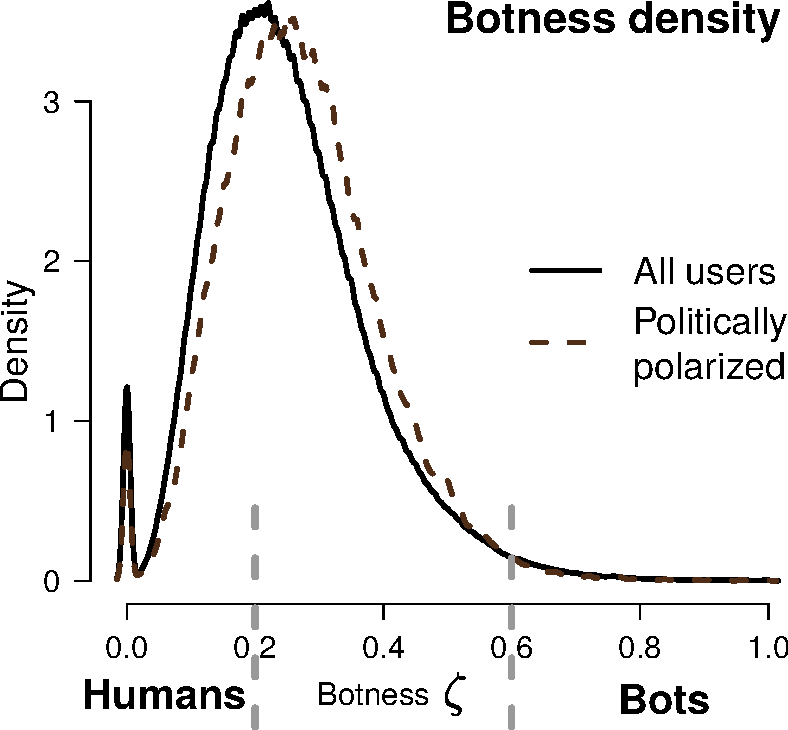
\includegraphics[height=\myheight\textheight]{botscore-density-all-polarization}
		\label{subfig:botscore-density}
	}
	\subfloat[] {
		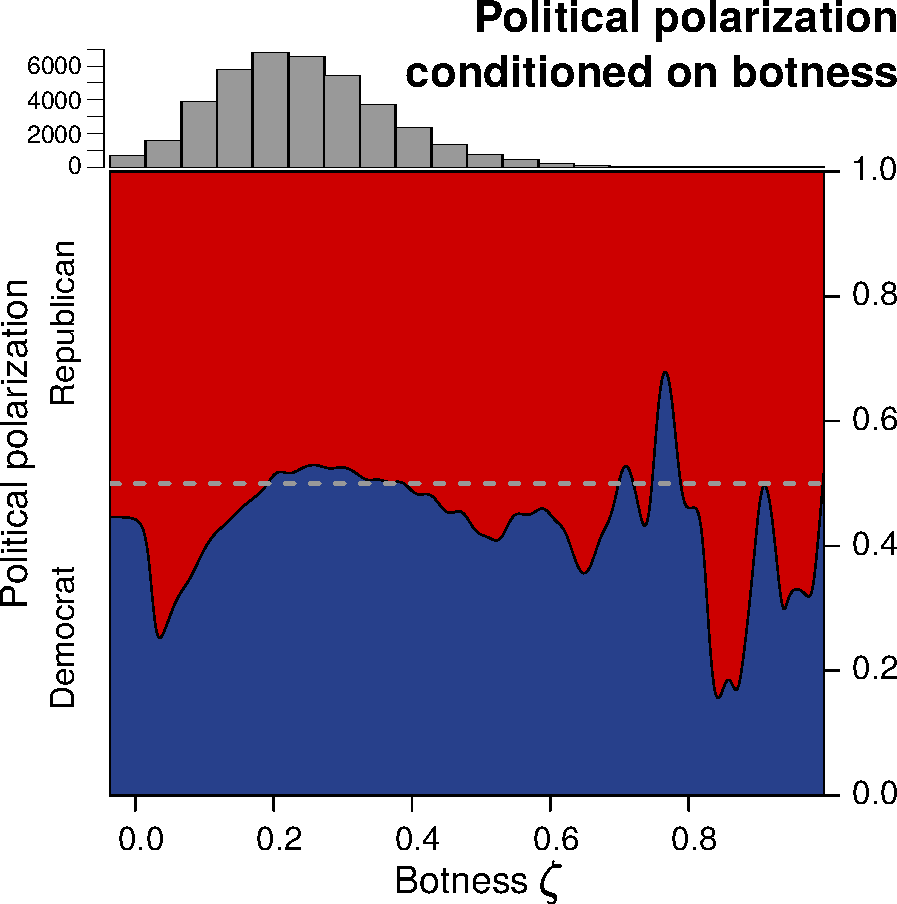
\includegraphics[height=\myheight\textheight]{botscore-conditional-density}
		\label{subfig:botscore-conditional-density}
	}}
	\\
	{ 
	\newcommand\myheight{0.145}
	\subfloat[] {
		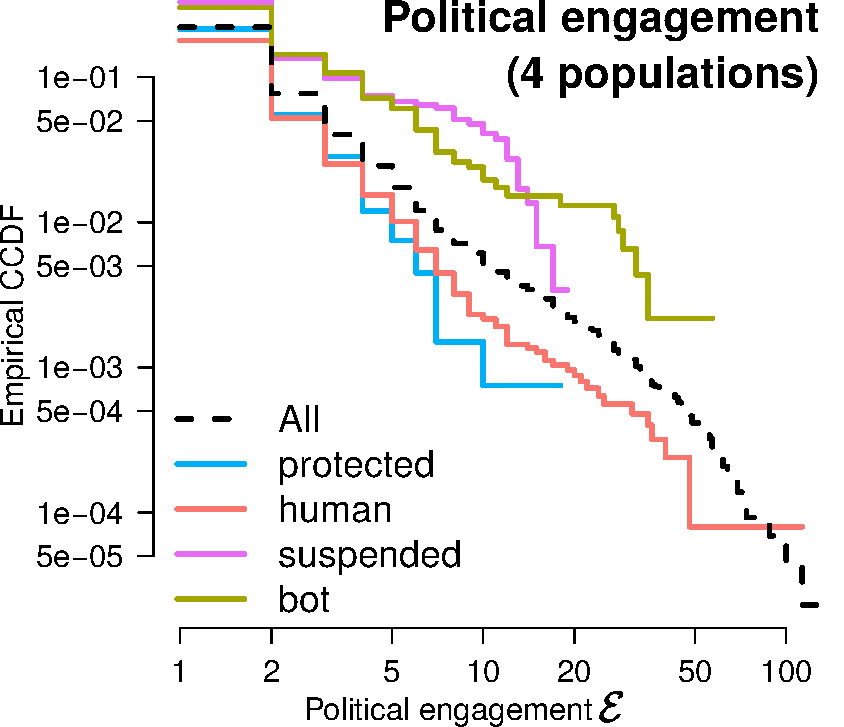
\includegraphics[height=\myheight\textheight]{c-pol-engagement-vs-botscore}
		\label{subfig:engagement-vs-botscore}
	}
	\subfloat[] {
		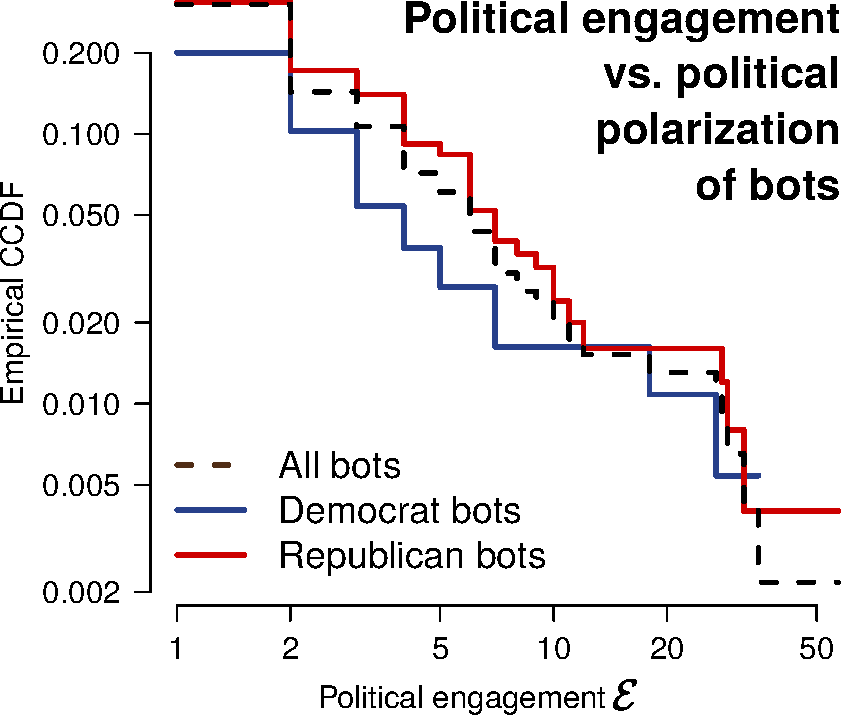
\includegraphics[height=\myheight\textheight]{d-BOTS_pol-engagement-vs-botscore}
		\label{subfig:BOTS_pol-engagement-vs-botscore}
	}
	}
	\caption{ 
		Political polarization, engagement and botness.
		\textbf{(a)} The density distribution of political polarization $\mathcal{P}$. %shows two peaks at -1 and 1, corresponding to strongly democrat and strongly republican respectively.
		\textbf{(b)} Log-log plot of the CCDF of political engagement $\mathcal{E}$ 
%		overall (dashed line), and 
		for the Democrat and Republican populations.
		% (blue and red lines respectively).
		%complementary cumulative distribution function shows that the political engagement score is long-tail distributed, with democrats being slightly more engaged than republicans overall.
		\textbf{(c)} The density distribution of botness $\zeta$ for the entire population (solid line) and the politically polarized population (dashed line). 
		%shows a large peak around $[0.1, 0.4]$ and a long tail.
		%Politically polarized users have slightly higher bot scores.
%		The dashed gray vertical lines show the threshholds for constructing the references human population ($\zeta \in [0, 0.2]$) and bot population ($\zeta \in [0.6, 1]$).
		\textbf{(d)} The conditional density of polarization conditioned on botness.
		The top panel shows the volumes of politically polarized users in 30 bins.
		\textbf{(e)(f)} CCDF of political engagement for the reference populations (e) and for the polarized \Bot populations (f).
		%\TODO{MAR}{Message in text: the \mbox{\Bot} and \mbox{\Suspended} populations are more politically engaged than the \mbox{\Human} and \mbox{\Protected}.}
	}
	\label{fig:bot-polarization}
%	\captionmoveup
\end{figure}